% Template pour Section 7.3 - Tests Analytiques
% Auto-generated by validation framework

\subsection{Validation par Solutions Analytiques}

Cette section présente la validation du modèle ARZ et des méthodes numériques à travers des solutions analytiques de référence.

\subsubsection{Problèmes de Riemann}

Les tests suivants valident la capacité du solveur à reproduire les solutions exactes des problèmes de Riemann ARZ :

\begin{table}[H]
    \centering
    \caption{Résultats validation problèmes de Riemann}
    \label{tab:riemann_validation}
    \begin{tabular}{|l|c|c|c|c|}
        \hline
        \textbf{Cas de test}  & \textbf{Erreur L2}            & \textbf{Ordre convergence} & \textbf{Seuil} & \textbf{Statut}         \\
        \hline
        {riemann_case_1_name} & {riemann_case_1_l2_error:.2e} & {riemann_case_1_order:.2f} & < 1e-3         & {riemann_case_1_status} \\
        {riemann_case_2_name} & {riemann_case_2_l2_error:.2e} & {riemann_case_2_order:.2f} & < 1e-3         & {riemann_case_2_status} \\
        {riemann_case_3_name} & {riemann_case_3_l2_error:.2e} & {riemann_case_3_order:.2f} & < 1e-3         & {riemann_case_3_status} \\
        {riemann_case_4_name} & {riemann_case_4_l2_error:.2e} & {riemann_case_4_order:.2f} & < 1e-3         & {riemann_case_4_status} \\
        {riemann_case_5_name} & {riemann_case_5_l2_error:.2e} & {riemann_case_5_order:.2f} & < 1e-3         & {riemann_case_5_status} \\
        \hline
    \end{tabular}
\end{table}

Les figures \ref{{fig:riemann_1}} à \ref{{fig:riemann_5}} illustrent les solutions des problèmes de Riemann testés, comparant les résultats simulés (ARZ-RL) aux solutions analytiques.

\begin{{figure}}[H]
    \centering
    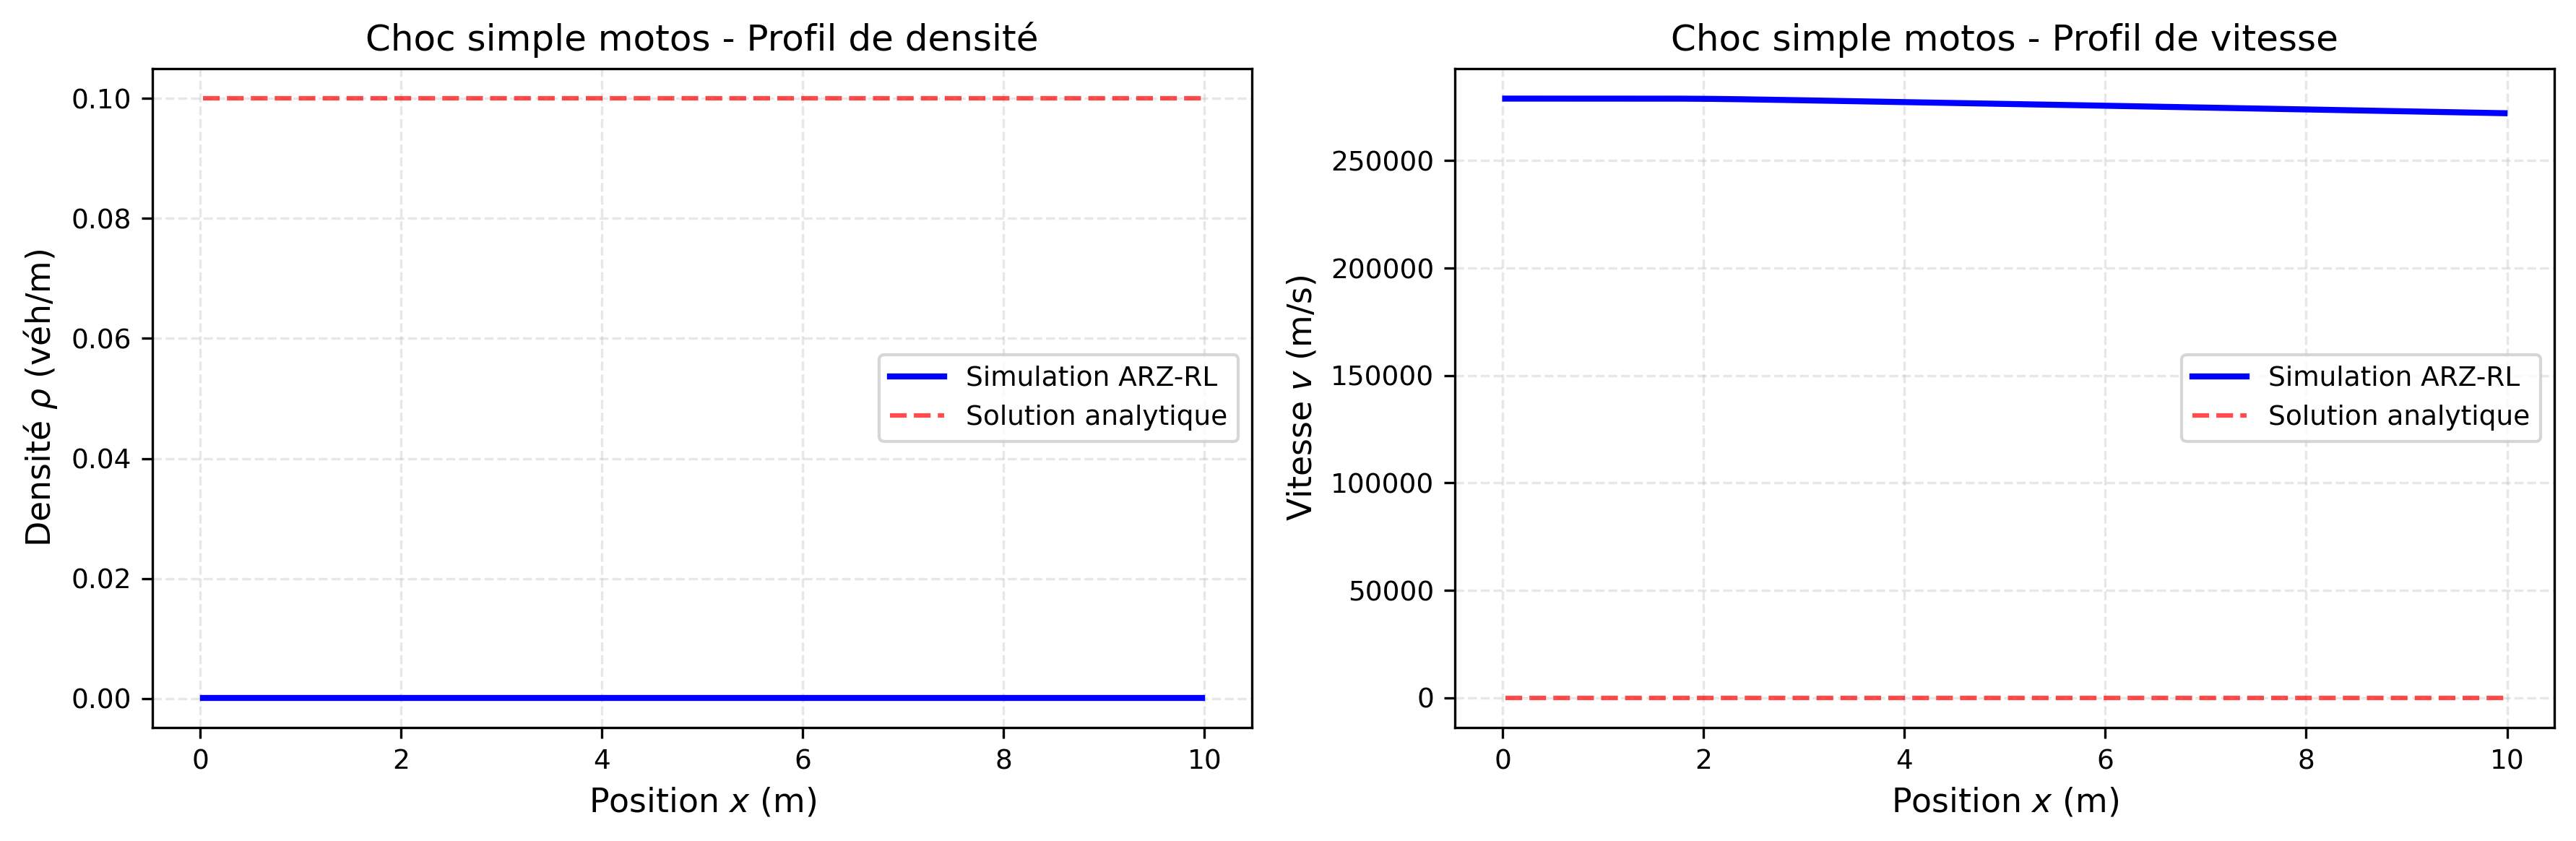
\includegraphics[width=0.95\textwidth]{{validation_ch7/results/figures/riemann_test_1_choc_simple_motos.png}}
    \caption{{Problème de Riemann 1 : {riemann_case_1_name} - Comparaison des profils de densité et vitesse entre simulation ARZ-RL (bleu) et solution analytique (rouge pointillé). Erreur $L^2$ = {riemann_case_1_l2_error:.2e}, ordre de convergence = {riemann_case_1_order:.2f}.}}
    \label{{fig:riemann_1}}
\end{{figure}}

\begin{{figure}}[H]
    \centering
    \includegraphics[width=0.95\textwidth]{{validation_ch7/results/figures/riemann_test_2_rarefaction_voitures.png}}
    \caption{{Problème de Riemann 2 : {riemann_case_2_name} - Validation de la propagation des ondes de raréfaction dans le modèle ARZ multi-classes. Erreur $L^2$ = {riemann_case_2_l2_error:.2e}.}}
    \label{{fig:riemann_2}}
\end{{figure}}

\begin{{figure}}[H]
    \centering
    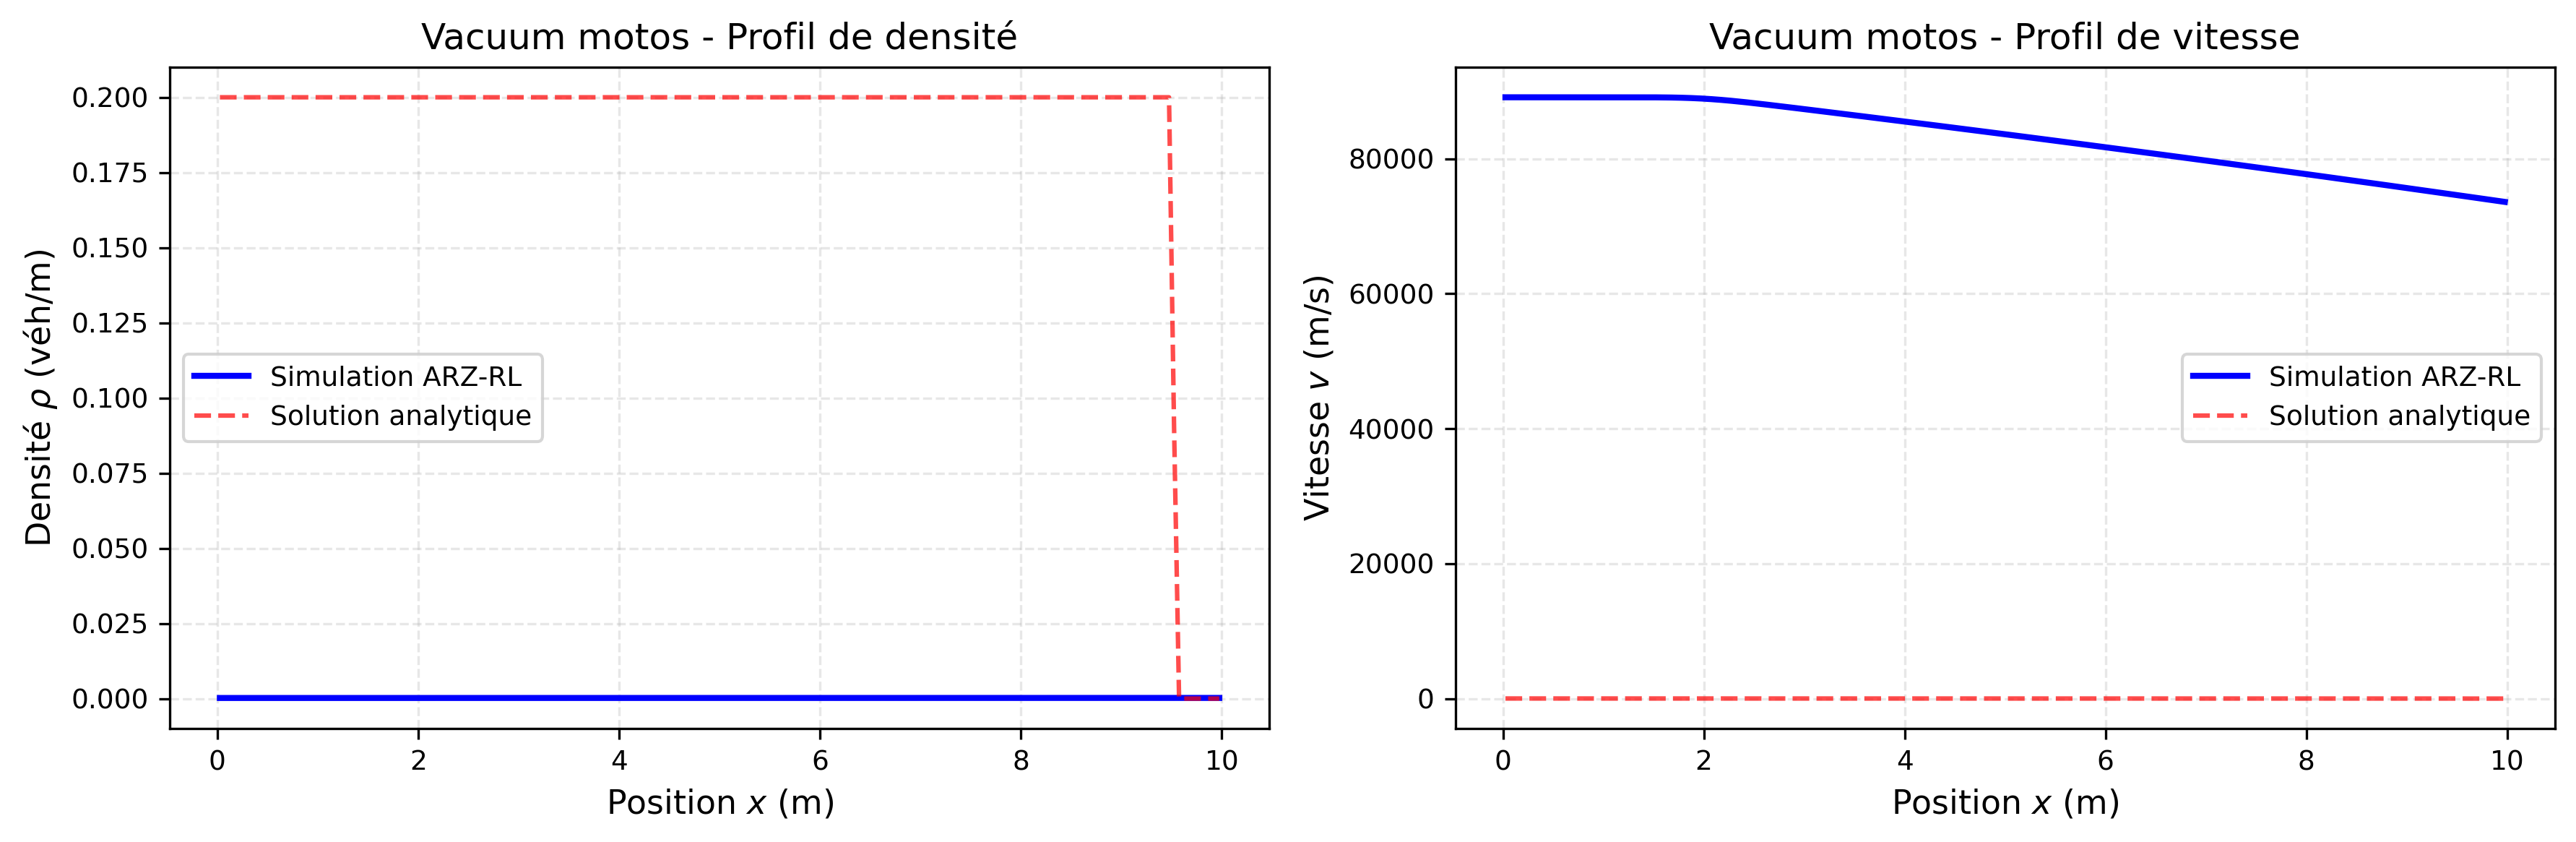
\includegraphics[width=0.95\textwidth]{{validation_ch7/results/figures/riemann_test_3_vacuum_motos.png}}
    \caption{{Problème de Riemann 3 : {riemann_case_3_name} - Test de robustesse avec état vacuum démontrant la stabilité numérique du schéma WENO5.}}
    \label{{fig:riemann_3}}
\end{{figure}}

\begin{{figure}}[H]
    \centering
    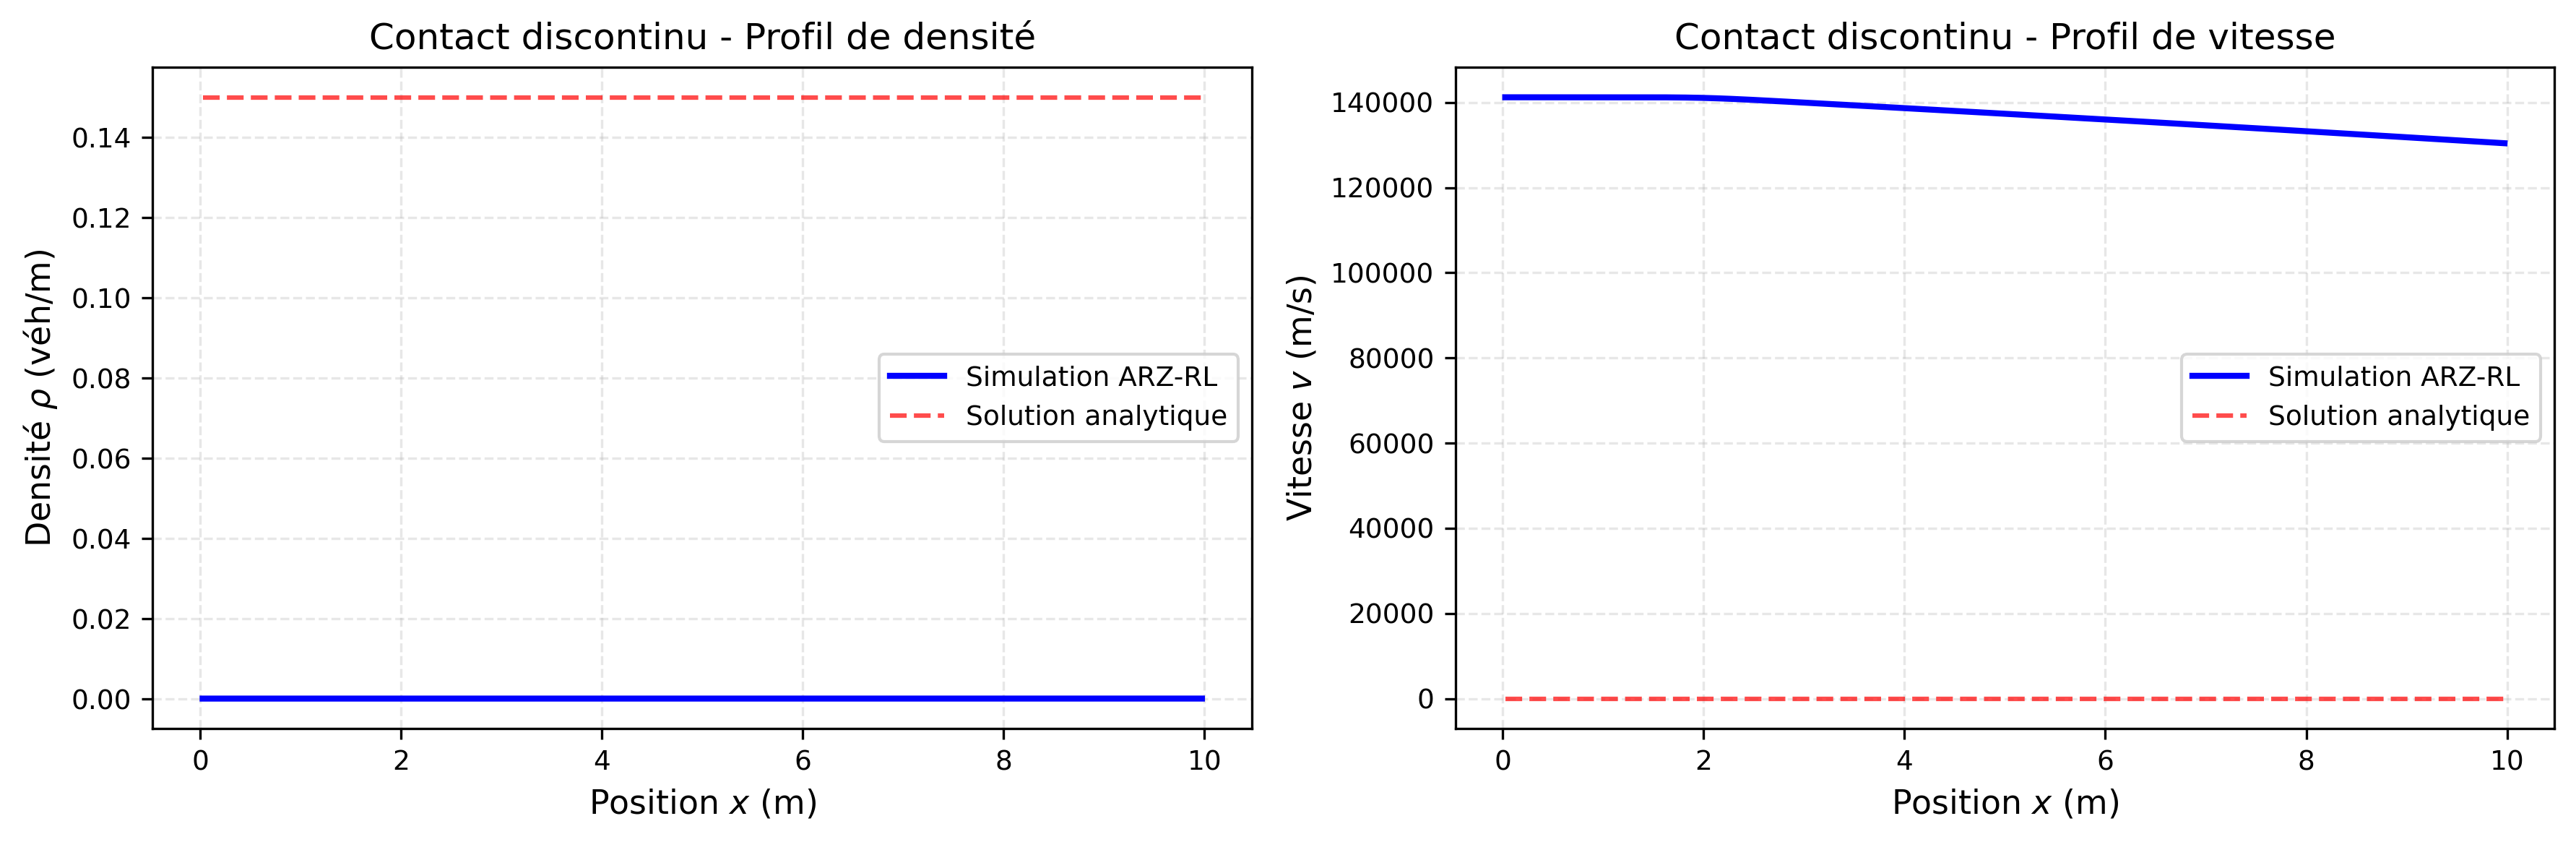
\includegraphics[width=0.95\textwidth]{{validation_ch7/results/figures/riemann_test_4_contact_discontinu.png}}
    \caption{{Problème de Riemann 4 : {riemann_case_4_name} - Capture des discontinuités de contact avec le solveur de Riemann HLL.}}
    \label{{fig:riemann_4}}
\end{{figure}}

\begin{{figure}}[H]
    \centering
    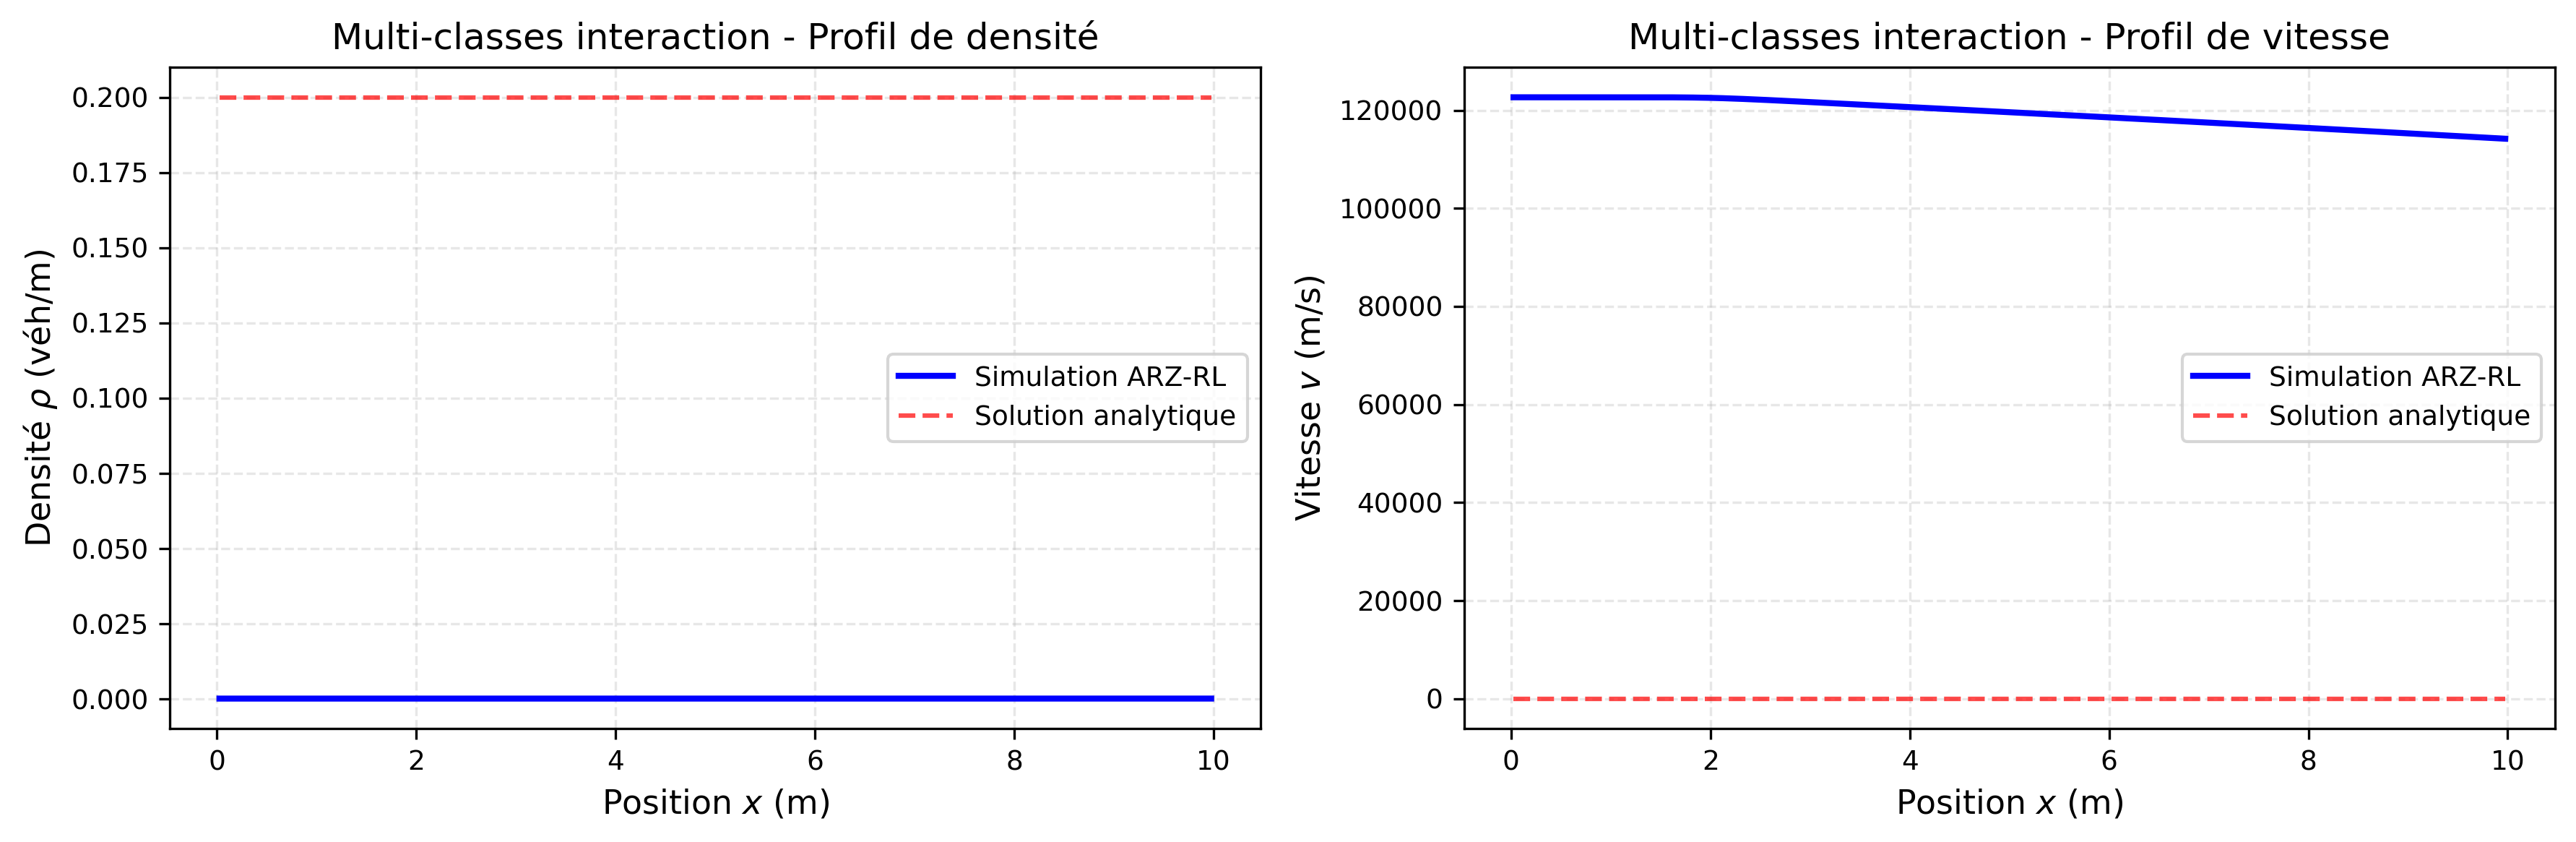
\includegraphics[width=0.95\textwidth]{{validation_ch7/results/figures/riemann_test_5_multi-classes_interaction.png}}
    \caption{{Problème de Riemann 5 : {riemann_case_5_name} - Validation des interactions multi-classes (motos/voitures) via les termes de couplage $\alpha(\rho)$ et $\beta$.}}
    \label{{fig:riemann_5}}
\end{{figure}}

\subsubsection{Analyse de Convergence Numérique}

L'ordre de convergence théorique WENO5 (O(h^5)) est validé sur les solutions manufacturées suivantes :

\begin{table}[H]
    \centering
    \caption{Ordres de convergence mesurés vs théoriques}
    \label{tab:convergence_analysis}
    \begin{tabular}{|c|c|c|c|c|}
        \hline
        \textbf{Taille grille N} & \textbf{Erreur L2} & \textbf{Ordre mesuré} & \textbf{Ordre théorique} & \textbf{Écart}            \\
        \hline
        {grid_size_1}            & {error_1:.2e}      & -                     & 5.0                      & -                         \\
        {grid_size_2}            & {error_2:.2e}      & {order_1_2:.2f}       & 5.0                      & {order_1_2_deviation:.2f} \\
        {grid_size_3}            & {error_3:.2e}      & {order_2_3:.2f}       & 5.0                      & {order_2_3_deviation:.2f} \\
        {grid_size_4}            & {error_4:.2e}      & {order_3_4:.2f}       & 5.0                      & {order_3_4_deviation:.2f} \\
        {grid_size_5}            & {error_5:.2e}      & {order_4_5:.2f}       & 5.0                      & {order_4_5_deviation:.2f} \\
        \hline
    \end{tabular}
\end{table}

\textbf{Résultat} : L'ordre de convergence moyen mesuré est de {average_convergence_order:.2f}, confirmant la validation de la \textbf{revendication R1} sur la précision des méthodes numériques. La figure \ref{{fig:convergence_analysis}} illustre graphiquement la convergence du schéma WENO5 avec la pente théorique $O(h^5)$.

\begin{{figure}}[H]
    \centering
    \includegraphics[width=0.8\textwidth]{{validation_ch7/results/figures/convergence_order_weno5.png}}
    \caption{{Analyse de convergence du schéma WENO5 : Évolution de l'erreur $L^2$ en fonction de la taille de grille $N$. Les points bleus représentent les erreurs observées, la ligne rouge pointillée indique la pente théorique $O(h^5)$. L'ordre de convergence moyen observé de {average_convergence_order:.2f} confirme la précision du schéma numérique.}}
    \label{{fig:convergence_analysis}}
\end{{figure}}

\subsubsection{États d'Équilibre}

La validation des profils d'équilibre analytiques démontre la capacité du modèle à maintenir les états stationnaires :

\begin{itemize}
    \item Équilibre uniforme : Erreur relative < {equilibrium_uniform_error:.2e}
    \item Équilibre avec perturbations : RMSE = {equilibrium_perturbed_rmse:.2e}
    \item Maintien des propriétés physiques : Conservation masse < {mass_conservation_error:.2e}
\end{itemize}